\documentclass[11pt,a4paper]{article}

\usepackage[utf8]{inputenc}
\usepackage[margin=2.2cm]{geometry}
\usepackage{amsmath,amssymb,amsthm}
\usepackage{booktabs}
\usepackage{graphicx}
\usepackage{tikz}
\usetikzlibrary{arrows.meta,positioning}
\usepackage[font=small,labelfont=bf]{caption}
\usepackage{microtype}
\usepackage[numbers,sort&compress]{natbib}
\usepackage[hidelinks]{hyperref}

\renewcommand{\topfraction}{0.92}\renewcommand{\bottomfraction}{0.85}
\renewcommand{\textfraction}{0.06}\renewcommand{\floatpagefraction}{0.88}
\setcounter{topnumber}{3}\setcounter{bottomnumber}{2}\setcounter{totalnumber}{5}
\newtheorem{theorem}{Theorem}
\newtheorem{observation}[theorem]{Observation}
\newcommand{\Vedge}{\textsc{V-edge}}
\newcommand{\Vclique}{\textsc{V-clique}}
\newcommand{\Estar}{\textsc{E-star}}
\DeclareMathOperator{\mad}{mad}

\title{Exact Coloring of Claw-Free Graphs:\\ The Role of Structural Representations}
\author{Aneta Wróblewska\\[2pt]
\small Maria Curie-Sk\l{}odowska University, Lublin, Poland\\
\small \texttt{aneta.wroblewska@umcs.pl}}
\date{}

\begin{document}
\maketitle

\begin{abstract}
\noindent
For a line graph $G=L(H)$ the chromatic number of $G$ equals the chromatic
index of the root graph $H$. We examine experimentally whether this fact helps
when $\chi(G)$ has to be computed exactly. We implemented in Python the
recognition of claw-free graphs and line graphs, the reconstruction of a root
graph, a DSATUR branch and bound, and three integer programming models solved
with HiGHS: an edge model and a maximal-clique model on $G$, and a star model
on the reconstructed root graph that uses Vizing's theorem. The implementation
was checked on all $5639$ connected claw-free graphs with at most nine
vertices. On $1125$ line graphs with up to $432$ vertices the root model was
faster than the edge model on $91\%$ of the instances (median speed-up $1.60$).
When the reconstruction time is included, it was faster on $71\%$ of the
instances (median speed-up $1.23$). The gain grows with the density of the root
graph and reaches a median of $6.6$ for the densest roots. Line graphs of
class~II roots were much harder for all methods. Among $240$ claw-free graphs
that are not line graphs, the complements of graphs produced by the random
triangle-free process were the hardest instances, although their chromatic
number can be found from a maximum matching.

\medskip\noindent
\textbf{Keywords:} claw-free graph, line graph, root graph, graph coloring,
edge coloring, DSATUR, integer programming, experimental algorithmics.
\end{abstract}

\section{Introduction}

A graph is \emph{claw-free} if it does not contain the star $K_{1,3}$ as an
induced subgraph. Line graphs are the best known claw-free graphs. Several
problems that are hard in general can be solved in polynomial time on
claw-free graphs, for example the maximum independent set problem
\cite{faudree1997}. Chudnovsky and Seymour developed a structure theory of the
class \cite{chudnovsky2005}, and claw-free graphs are often used to test
conjectures on the relation between $\chi$, $\omega$ and $\Delta$
\cite{scott2020,cook2025}.

Vertex coloring stays hard on this class. For a line graph $G=L(H)$, a proper
vertex coloring of $G$ is the same as a proper edge coloring of $H$, so
$\chi(L(H))=\chi'(H)$. Holyer \cite{holyer1981} proved that it is NP-complete to
decide whether a cubic graph has chromatic index~$3$. Hence computing $\chi$ is
NP-hard already for line graphs.

On the other hand, the root graph gives useful information. By Vizing's
theorem \cite{vizing1964}, $\chi'(H)\in\{\Delta(H),\Delta(H)+1\}$, and by
K\"onig's theorem \cite{konig1916}, $\chi'(H)=\Delta(H)$ for bipartite $H$. A
root graph can be reconstructed in time linear in the size of $G$
\cite{roussopoulos1973,liu2015}. It is therefore natural to ask whether an
exact solver should color the vertices of $G$ directly, or first reconstruct
$H$ and color its edges. We study this question together with two related
ones:
\begin{description}\setlength{\itemsep}{1pt}
\item[RQ1.] How does the difficulty of exact coloring differ between the
selected families of line graphs and of claw-free graphs that are not line
graphs?
\item[RQ2.] Does the root-graph representation of $G=L(H)$ reduce the time
needed to compute $\chi(G)$ exactly?
\item[RQ3.] Which structural parameters are most strongly associated with the
running time of the exact methods?
\end{description}
Our working hypotheses were: (H1) for many line graphs, edge coloring of $H$ is
faster than vertex coloring of $L(H)$; (H2) the gain grows with
$R=|E(H)|/|V(H)|=|V(L(H))|/|V(H)|$; (H3) the chromatic gap $\chi(G)-\omega(G)$,
the degeneracy and the local neighborhood density are more closely related to
the difficulty than the number of vertices.

The paper does not propose a new coloring algorithm. Its contribution is an
experimental comparison of several formulations of the same problem on the same
instances, a set of test families with known properties, and an analysis of how
the structure of a graph is related to the cost of exact coloring.

\subsection{Related work}

\paragraph{Coloring claw-free graphs.}
Chudnovsky and Seymour \cite{chudnovsky2010} proved that $\chi\le 2\omega$ for
every connected claw-free graph with $\alpha\ge 3$. Such bounds are studied
within the theory of $\chi$-boundedness \cite{scott2020}; for example,
$\chi\le\lceil 3\omega/2\rceil$ holds for graphs without an induced fork and
without $C_4$ \cite{chudnovsky2021}. Recently, Vu's conjecture, which bounds
$\chi$ in terms of the maximum number of common neighbors of two vertices,
was proved for claw-free graphs \cite{cook2025}. Our experiments cover two
very different parts of the class: line graphs, where $\chi\le\omega+1$, and
complements of triangle-free graphs ($\alpha\le 2$), where the gap
$\chi-\omega$ can be large.

\paragraph{Edge coloring.}
A survey of results up to 2019 is given in \cite{cao2019}. Since then the
Goldberg--Seymour conjecture for multigraphs has been proved \cite{chen2025}.
For simple graphs the main open question is the Overfull Conjecture: a graph
with $\Delta>n/3$ should be of class~II exactly when it contains an overfull
subgraph with the same maximum degree. It has been confirmed for several
families of dense graphs \cite{cao2022}. A $(\Delta+1)$-edge-coloring can be
found in near-linear time \cite{assadi2025}, and Kowalik \cite{kowalik2024}
gave a quasilinear algorithm for $\Delta$-edge-coloring when
$\Delta\ge 2\mad(H)$, where $\mad(H)$ is the maximum average degree of a
subgraph of $H$. So the upper bound in Vizing's theorem is cheap to reach, and
the hard part of exact edge coloring is to decide the class of the graph. This
is what the root model in our study has to do.

\paragraph{Exact vertex coloring.}
Classical exact methods are DSATUR-based branch and bound
\cite{brelaz1979,sansegundo2012,furini2017} and integer programming with the
assignment formulation strengthened by clique constraints
\cite{mendez2006,malaguti2010}. Newer approaches use decision diagrams
\cite{vanhoeve2022}, SAT encodings of partial-ordering models
\cite{faber2024} and SAT procedures that alternate between cliques and
colorings \cite{heule2022}. These methods are usually tested on the DIMACS
benchmark and on random graphs. Structured classes such as line graphs, for
which the instance has a second representation, are not considered there. We
did not find a study that compares, on the same instances, vertex coloring of
line graphs with edge coloring of their reconstructed roots.

\section{Preliminaries}

All graphs are finite and simple. For a graph $G$ we write $n=|V(G)|$,
$m=|E(G)|$, $\Delta(G)$ for the maximum degree, $\omega(G)$ for the clique
number, $\alpha(G)$ for the independence number, $\chi(G)$ for the chromatic
number and $\chi'(G)$ for the chromatic index. The \emph{line graph} $L(H)$ has
vertex set $E(H)$, and two vertices are adjacent if the corresponding edges of
$H$ share an endpoint; $H$ is a \emph{root graph} of $L(H)$.

\paragraph{Claw-free graphs and line graphs.}
A graph is claw-free if and only if $\alpha(G[N(v)])\le 2$ for every vertex $v$.
Every line graph is claw-free, since three pairwise non-adjacent neighbors of
a vertex $xy$ of $L(H)$ would be three disjoint edges of $H$, each meeting
$\{x,y\}$. Beineke \cite{beineke1970} characterized line graphs by nine
forbidden induced subgraphs, one of which is the claw. We use the older
characterization of Krausz (see \cite{beineke1970,liu2015}): $G$ is a line
graph if and only if its edges can be partitioned into cliques so that every
vertex lies in at most two of them. In $L(H)$ such a partition is formed by the
\emph{stars} of $H$, that is, by the sets of edges incident with a vertex of
$H$. By Whitney's theorem (see \cite{liu2015}), a connected line graph other
than $K_3$ has a unique root graph without isolated vertices. The graph $K_3$
has two roots, $K_3$ and $K_{1,3}$; both have chromatic index $3$, so the choice
does not change the result, although it changes the star model.

\paragraph{Coloring.}
The stars of $H$ are cliques of $L(H)$, so $\omega(L(H))\ge\Delta(H)$, and
Vizing's theorem gives
\begin{equation}\label{eq:vizing}
\Delta(H)\le\chi'(H)=\chi(L(H))\le\Delta(H)+1\le\omega(L(H))+1 .
\end{equation}
A graph $H$ is of \emph{class~I} if $\chi'(H)=\Delta(H)$ and of \emph{class~II}
otherwise. Bipartite graphs are of class~I \cite{konig1916}, and almost all
graphs are of class~I \cite{erdos1977}. A graph $H$ is \emph{overfull} if
$|E(H)|>\Delta(H)\lfloor |V(H)|/2\rfloor$. An overfull graph is of class~II,
because each color class is a matching and has at most
$\lfloor |V(H)|/2\rfloor$ edges. In particular, a $d$-regular graph of odd
order with $d\ge 1$ is overfull; by the handshake lemma $d$ must then be even.

For general claw-free graphs the gap $\chi-\omega$ can exceed one. Graphs with
$\alpha(G)\le 2$ are exactly the complements of triangle-free graphs, and they
are claw-free. If $T$ is triangle-free and $G=\overline{T}$, then a color class
of $G$ is a clique of $T$, i.e.\ a vertex or an edge. Therefore
\begin{equation}\label{eq:matching}
\chi(\overline{T})=|V(T)|-\nu(T),\qquad \omega(\overline{T})=\alpha(T),
\end{equation}
where $\nu(T)$ is the size of a maximum matching. An optimal coloring is
obtained by giving one color to the two ends of each matching edge and a
separate color to every other vertex. Both $\chi$ and an optimal coloring can
thus be found in polynomial time, which gives an independent check of the
solvers. If $T$ is bipartite, then $\nu(T)=|V(T)|-\alpha(T)$ by K\"onig's
theorem and $\chi(\overline{T})=\omega(\overline{T})$.

\section{Algorithms and implementation}

The software is written in Python. It uses NetworkX \cite{hagberg2008} for
graphs, SciPy \cite{virtanen2020} for statistics and as the interface to the
HiGHS solver \cite{huangfu2018}, and Matplotlib for plots. The course of the
main experiment is shown in Figure~\ref{fig:scheme}.

\begin{figure}[!tb]
\centering
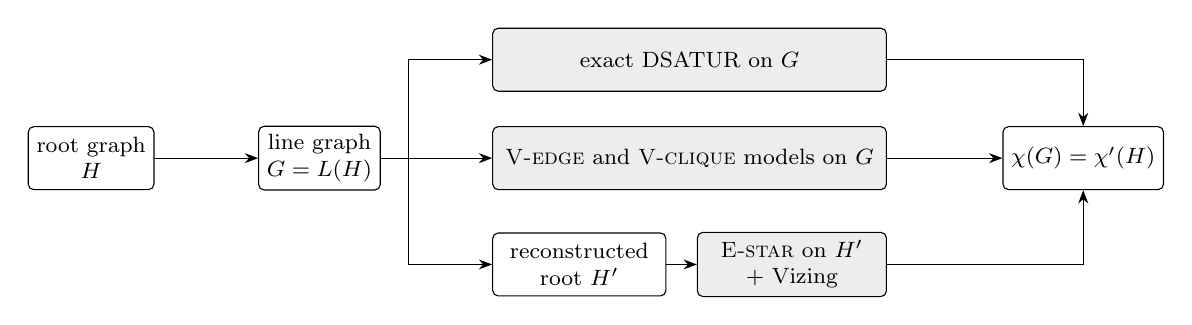
\begin{tikzpicture}[>=Stealth, font=\footnotesize,
  box/.style={draw, rounded corners=2pt, align=center, inner sep=3pt, minimum height=8mm},
  alg/.style={box, fill=black!7}]
\node[box] (H) at (0,0) {root graph\\$H$};
\node[box] (G) at (2.9,0) {line graph\\$G=L(H)$};
\node[alg, minimum width=50mm] (D) at (7.6,1.25) {exact DSATUR on $G$};
\node[alg, minimum width=50mm] (V) at (7.6,0) {\Vedge{} and \Vclique{} models on $G$};
\node[box, minimum width=22mm] (R) at (6.2,-1.35) {reconstructed\\root $H'$};
\node[alg, minimum width=24mm] (E) at (8.9,-1.35) {\Estar{} on $H'$\\+ Vizing};
\node[box] (X) at (12.6,0) {$\chi(G)=\chi'(H)$};
\draw[->] (H) -- (G);
\draw[->] (G) -- (V);
\draw[->] (G.east) ++(3.5mm,0) |- (D.west);
\draw[->] (G.east) ++(3.5mm,0) |- (R.west);
\draw[->] (R) -- (E);
\draw[->] (V) -- (X);
\draw[->] (D.east) -| (X.north);
\draw[->] (E.east) -| (X.south);
\end{tikzpicture}
\caption{Scheme of the main experiment. The solvers receive only the line
graph $G$ with randomly permuted vertices; the root graph used by the star
model is reconstructed from $G$.}
\label{fig:scheme}
\end{figure}

\paragraph{Recognition.}
Claw-freeness is tested from the definition: for every vertex $v$ and every
pair $a,b$ of non-adjacent neighbors of $v$ we look for a neighbor of $v$
adjacent to neither $a$ nor $b$. A claw found in this way is returned as a
certificate. Line graphs are recognized by reconstructing a root graph with the
algorithm of Roussopoulos \cite{roussopoulos1973} as implemented in NetworkX,
applied to each connected component. The result is then checked: the
reconstruction gives a map $\varphi\colon V(G)\to E(H')$, and we verify that
$\varphi$ is a bijection and that $uv\in E(G)$ if and only if $\varphi(u)$ and
$\varphi(v)$ share an endpoint. For a component equal to $K_3$ the
implementation returns the root $K_{1,3}$. The map $\varphi$ also turns an edge
coloring of $H'$ into a vertex coloring of $G$.

\paragraph{Structural parameters.}
For every graph we compute $n$, $m$, the density $2m/(n(n-1))$, the minimum,
maximum and average degree, the degeneracy, the number of triangles, the clique
number (by enumerating maximal cliques) and the mean neighborhood density
$D_N(G)=\frac1{n}\sum_{v}D_N(v)$, where $D_N(v)=|E(G[N(v)])|/\binom{d(v)}{2}$
for $d(v)\ge 2$ and $D_N(v)=0$ otherwise. $D_N$ is the average local clustering
coefficient and is used only as a descriptor of local structure. In a
claw-free graph the complement of every neighborhood is triangle-free, so by
Mantel's theorem the neighborhood of a vertex of large degree has density
at least about $1/2$. Hence $D_N$ is high on claw-free graphs.

\paragraph{Exact DSATUR.}
The first exact method is the DSATUR branch and bound of Br\'elaz
\cite{brelaz1979}. It selects an uncolored vertex of maximum saturation degree
(ties are broken by degree) and tries every admissible color already in use
and one new color, as long as the number of colors stays below the best
solution found so far. The initial upper bound is given by the greedy DSATUR
heuristic and the lower bound is $\omega(G)$; the search stops when the two
bounds meet. We record the running time and the number of nodes of the search
tree. The node count does not depend on the load of the machine, but it does
depend on the branching rule and the bounds used.

\paragraph{Integer programming models.}
The other methods solve a sequence of $k$-colorability problems with the
assignment formulation \cite{mendez2006}. Let $I$ be the set of items to be
colored and $\mathcal{Q}$ a family of sets of items whose members must get
different colors. With binary variables $x_{ic}$ ($i\in I$, $0\le c<k$) we look
for a solution of
\begin{equation}\label{eq:ilp}
\sum_{c<k}x_{ic}=1\quad(i\in I),\qquad
\sum_{i\in Q}x_{ic}\le 1\quad(Q\in\mathcal{Q},\ c<k).
\end{equation}
The three models differ only in $I$ and $\mathcal{Q}$:
\begin{itemize}\setlength{\itemsep}{1pt}
\item \Vedge: $I=V(G)$ and $\mathcal{Q}=E(G)$; no structural information is used.
\item \Vclique: $I=V(G)$ and $\mathcal{Q}$ is the family of all maximal cliques
of $G$, found by the Bron--Kerbosch procedure in NetworkX. The time of this
enumeration is included in the running time of the model.
\item \Estar: $I=E(H')$ and $\mathcal{Q}$ is the family of stars of the
reconstructed root $H'$, i.e.\ the Krausz partition of $G$. This model is
applied only to line graphs.
\end{itemize}
In the vertex models the colors of a maximum clique are fixed to remove the
symmetry between colors, and $k=\omega(G),\omega(G)+1,\dots$ is tested until a
coloring is found. In \Estar{} the colors of the edges at a vertex of maximum
degree are fixed and only $k=\Delta(H')$ is tested; if this model is infeasible,
then $\chi'(H')=\Delta(H')+1$ by~\eqref{eq:vizing}. For class~I roots the model
returns an optimal edge coloring, which is mapped back to $G$. For class~II
roots it determines the exact value of $\chi(G)$ but does not construct a
coloring with $\Delta(H')+1$ colors; such a coloring can be found by a
randomized near-linear-time algorithm \cite{assadi2025}, but this step is not part of the measured
procedure, whereas the vertex models always return a coloring. We do not use other
shortcuts, such as K\"onig's theorem or the overfull test, so that the
comparison concerns the models themselves.

An edge model of $H$ with one constraint for every pair of adjacent edges
would be identical to \Vedge{}. The root graph can therefore help only through
the clique (star) constraints and through the bound~\eqref{eq:vizing}. The
star constraints are also much fewer: \Vedge{} has
$k\sum_{v\in V(H)}\binom{d_H(v)}{2}$ conflict rows and \Estar{} at most
$k|V(H)|$. The \Vclique{} model separates the effect of clique constraints,
which can be obtained without the root graph, from the effect of the
reconstruction and of Vizing's bound.

Every coloring returned by a solver is checked, and the results of all methods
on the same graph are compared.

\section{Test instances}

All instances were generated with fixed random seeds; the generators, the
seeds and the resulting graphs are included in the repository given at the end
of the paper.

\paragraph{Set A: line graphs.}
A root graph $H$ is generated, $G=L(H)$ is formed and the vertices of $G$ are
randomly permuted. We use five families of roots and $15$ graphs for each
selected parameter combination. Erd\H{o}s--R\'enyi graphs $G(n,p)$ have
$n\in\{10,20,30,40,50\}$ and $p=\bar d/(n-1)$ for the expected average degree
$\bar d\in\{2,4,8,16\}$; only combinations satisfying $\bar d\le n-2$ were included;
isolated vertices are removed. Random bipartite graphs have parts of sizes
$\lfloor n/2\rfloor$ and $\lceil n/2\rceil$, the same $n$, and edge
probability $p=\bar d n/(2\lfloor n/2\rfloor\lceil n/2\rceil)$; here only
combinations with $\bar d<n/2$ were included. Trees are uniformly random labeled trees on the same numbers of
vertices. Random $d$-regular graphs \cite{steger1999} have $d\in\{3,4,6,8\}$ and
$n\in\{10,15,20,25,30,40,50\}$, excluding odd $nd$. Finally,
\emph{subdivided regular graphs} are obtained from a random $d$-regular graph
of odd order $n_0\in\{15,25,35\}$, $d\in\{4,6,8\}$, by subdividing one edge. The
regular graphs of odd order are overfull. The subdivided ones give class~II
roots that are not overfull:

\begin{observation}\label{obs:subdiv}
Let $d\ge 3$, let $F$ be a $d$-regular graph of odd order and let $H$ be
obtained from $F$ by subdividing one edge. Then $H$ is of class~II and is not
overfull.
\end{observation}
\begin{proof}
Let $w$ be the new vertex. In an edge coloring of $H$ with $d=\Delta(H)$
colors every vertex of degree $d$ meets every color class. A color class is a
matching, so it covers an even number of vertices; since $|V(F)|$ is odd, it
must also cover $w$. Then all $d\ge 3$ colors appear at $w$, which has degree
two, a contradiction. Finally,
$|E(H)|=d|V(F)|/2+1\le d(|V(F)|+1)/2=\Delta(H)\lfloor|V(H)|/2\rfloor$.
\end{proof}

\noindent
Although $H$ is not overfull, it contains an overfull subgraph with the same
maximum degree, namely $H-w$. This is the kind of obstruction described by the
Overfull Conjecture \cite{cao2022}.

\paragraph{Set B: claw-free graphs that are not line graphs.}
By~\eqref{eq:matching}, complements of triangle-free graphs are claw-free and
their chromatic number is known. We use two families with
$n\in\{20,30,40,50\}$ and $30$ graphs per value of $n$. \emph{Co-bipartite}
graphs are complements of random balanced bipartite graphs with edge
probability $0.3$ or $0.6$. \emph{Co-triangle-free} graphs are complements of
graphs produced by the triangle-free process (pairs of vertices are taken in
random order, and an edge is added if it does not close a triangle), run to the
end or stopped after half of its edges. None of the $240$ graphs is a line
graph. This set is a control group, not a sample of all claw-free graphs: its
graphs are dense and have $\alpha\le 2$.

\paragraph{Set C: all small claw-free graphs.}
All connected claw-free graphs with at most nine vertices were generated up to
isomorphism by adding one vertex at a time and removing isomorphic copies. This
is enough, because every connected graph has a vertex whose removal leaves it
connected, and claw-freeness is hereditary. The numbers obtained,
$1,1,2,5,14,50,191,881,4494$ for $n=1,\dots,9$, and the numbers of line graphs
among them, $1,1,2,5,12,30,79,227,710$, agree with the sequences A022562 and
A003089 of the OEIS \cite{oeis}. Table~\ref{tab:sets} summarizes the three sets.

\begin{table}[!tb]
\centering\small
\caption{Test sets; $n$ and $m$ refer to the colored graph $G$. In set A only the
parameter combinations described in the text were generated.}
\label{tab:sets}
\begin{tabular}{llrrrrr}
\toprule
Set & Family & Graphs & $n$ & $m$ & Mean density & Line graphs\\
\midrule
A & Erd\H{o}s--R\'enyi & 285 & 4--432 & 3--7250 & 0.16 & 285\\
A & bipartite & 240 & 4--415 & 2--6598 & 0.14 & 240\\
A & trees & 75 & 9--49 & 9--83 & 0.14 & 75\\
A & regular & 390 & 15--200 & 30--1400 & 0.15 & 390\\
A & subdivided regular & 135 & 31--141 & 91--981 & 0.15 & 135\\
\midrule
B & co-bipartite & 120 & 20--50 & 120--1060 & 0.77 & 0\\
B & co-triangle-free & 120 & 20--50 & 109--1081 & 0.78 & 0\\
\midrule
C & line & 1067 & 1--9 & 0--36 & 0.45 & 1067\\
C & non-line & 4572 & 5--9 & 7--35 & 0.62 & 0\\
\bottomrule
\end{tabular}

\end{table}

\section{Experimental methodology}

The experiments were run on one machine (two cores of an Intel Xeon processor
at 2.3\,GHz, 7\,GB of memory, Linux) with Python~3.13.16, NetworkX~3.6.1,
NumPy~2.5.3 and SciPy~1.18.1. The \texttt{milp} routine of SciPy calls HiGHS
with default settings. Two instances were processed at the same time in two
separate processes. Each method had a limit of $30$\,s per graph. For the
vertex models this limit covers the whole sequence of $k$-colorability
problems, and each call to the solver receives the remaining time. Times of
the models include building the constraint matrix. For a run that reached the
limit, we record the measured time, which can exceed the limit slightly
(by at most $0.05$\,s in our runs) because the limit is checked only
periodically; the node count of DSATUR is the value at the moment of
interruption. Medians of times and node counts are
taken over all instances, including such runs.

We denote by $T_V$, $T_C$ and $T_E$ the times of \Vedge, \Vclique{} and \Estar,
by $T_{\mathrm{rec}}$ the time of the root reconstruction, and define
\[
S=\frac{T_V}{T_E},\qquad S_{\mathrm{tot}}=\frac{T_V}{T_E+T_{\mathrm{rec}}} .
\]
$S$ compares the two models, and $S_{\mathrm{tot}}$ also charges the root model
with the cost of reconstruction. The time needed to compute $\omega(G)$ is
common to DSATUR and the vertex models and is not included in $T_V$ and $T_C$;
this slightly favors the vertex models.

Groups are described by medians and, for ratios, by geometric means. Paired
samples are compared with the Wilcoxon signed-rank test, independent samples
with the Mann--Whitney test, and associations are measured by Spearman's
rank correlation $\rho$. Graphs generated with the same parameters are not
independent in the sense of a random sample from all claw-free graphs, so the
tests describe the generated families and should not be read as statements
about the whole class. Many times are of the order of milliseconds and are
affected by measurement noise; for this reason we rely on medians and rank
statistics.

\section{Results}

\begin{table}[!htb]
\centering\small
\caption{Structural parameters (means unless stated otherwise). For set B the
chromatic number is taken from~\eqref{eq:matching}.}
\label{tab:params}
\begin{tabular}{llrrrrrrr}
\toprule
Set & Family & $\omega$ & $\chi$ & $\chi>\omega$ [\%] & $\max(\chi-\omega)$ & $\max\chi/\omega$ & Degen. & $D_N$\\
\midrule
A & Erd\H{o}s--R\'enyi & 11.2 & 11.2 & 0.0 & 0 & 1.00 & 11.0 & 0.50\\
A & bipartite & 9.2 & 9.2 & 0.0 & 0 & 1.00 & 9.1 & 0.46\\
A & trees & 4.2 & 4.2 & 0.0 & 0 & 1.00 & 3.2 & 0.40\\
A & regular & 5.4 & 5.7 & 23.3 & 1 & 1.33 & 8.8 & 0.44\\
A & subdivided regular & 6.0 & 7.0 & 100.0 & 1 & 1.25 & 9.0 & 0.46\\
\midrule
B & co-bipartite & 17.6 & 17.6 & 0.0 & 0 & 1.00 & 22.5 & 0.80\\
B & co-triangle-free & 13.3 & 17.5 & 94.2 & 11 & 1.79 & 24.1 & 0.80\\
\midrule
C & line & 3.9 & 4.0 & 0.7 & 1 & 1.50 & 3.0 & 0.54\\
C & non-line & 4.7 & 4.8 & 8.7 & 1 & 1.33 & 4.0 & 0.67\\
\bottomrule
\end{tabular}

\end{table}

\begin{figure}[!htb]
\centering
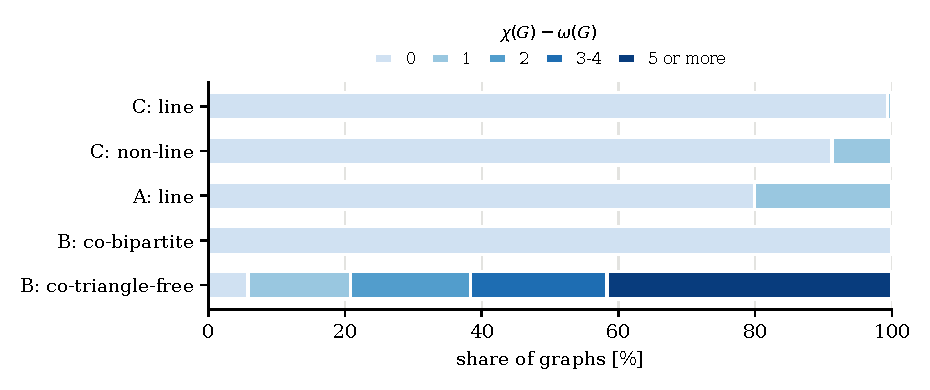
\includegraphics[width=0.56\textwidth]{figures/fig_gap}
\caption{Distribution of the chromatic gap $\chi(G)-\omega(G)$.}
\label{fig:gap}
\end{figure}

\subsection{Validation}

On set C, DSATUR and \Vedge{} solved all $5639$ graphs and returned the same
chromatic number. On the $1067$ line graphs of this set, \Vclique{} and \Estar{}
gave the same values as well, which confirms $\chi(G)=\chi'(H')$ for the
reconstructed roots. On set B, the values found by DSATUR ($180$ solved graphs)
and by \Vedge{} ($216$ solved graphs) always agreed with
$|V(T)|-\nu(T)$ from~\eqref{eq:matching}. On set A all methods agreed on every
instance solved by more than one of them. We found no inconsistent result.

\subsection{Structural properties}

Table~\ref{tab:params} and Figure~\ref{fig:gap} describe the instances. Every
connected claw-free graph with at most nine vertices satisfies
$\chi\le\omega+1$. The gap is positive for $406$ of them, and only $7$ of these
are line graphs (the line graphs of class~II roots, e.g.\ $C_5=L(C_5)$). So
among small claw-free graphs, $\chi>\omega$ is much more frequent outside the
class of line graphs ($8.7\%$ against $0.7\%$).

In set A the gap is positive exactly for class~II roots, as \eqref{eq:vizing}
predicts. All Erd\H{o}s--R\'enyi, bipartite and tree roots were of class~I,
which agrees with \cite{erdos1977,konig1916}. Co-bipartite graphs are perfect,
whereas co-triangle-free graphs have the largest gaps (mean $4.2$, maximum
$11$, $\chi/\omega$ up to $1.79$). As expected, $D_N$ is high in all sets.

\subsection{Line graphs and non-line claw-free graphs (RQ1)}

Table~\ref{tab:solvers} and Figure~\ref{fig:time} compare DSATUR and the
\Vedge{} model on all sets. When the greedy DSATUR coloring already uses
$\omega(G)$ colors, the instance is solved without search. This happened for
almost all line graphs of Erd\H{o}s--R\'enyi, bipartite and tree roots and for
$96\%$ of the co-bipartite graphs. When $\chi>\omega$, the branch and bound has
to prove a lower bound, and the search tree grows very quickly. DSATUR reached
the time limit on $173$ line graphs ($165$ of them with class~II roots) and on
half of the co-triangle-free graphs. The \Vedge{} model is slower on easy
instances because of a fixed overhead of a few milliseconds. With the tested
implementations, however, it was clearly more reliable than our Python DSATUR
on instances with $\chi>\omega$: it solved all graphs of set A and $80\%$ of the
co-triangle-free graphs.

To compare graphs of similar size we restricted set A to $20\le n\le 50$ ($362$
graphs). In this range DSATUR solved $91.7\%$ of the line graphs and $75.0\%$ of
the graphs of set B, and \Vedge{} solved $100\%$ and $90.0\%$. The median of
$T_V$ was $7.3$\,ms against $27.6$\,ms (Mann--Whitney test, $p<10^{-40}$). The
difference comes from the co-triangle-free family. Its gap can be large, so the
vertex models need on average $4.8$ solver calls per graph, most of them
infeasible. None of the complements of maximal triangle-free graphs on $50$
vertices was solved by either method, although their chromatic number follows
from a maximum matching. The two sets also differ in density ($0.19$ against
$0.77$ in this range), so the result describes the tested families only.

\begin{table}[!tb]
\centering\small
\caption{Exact DSATUR and the \Vedge{} model (time limit $30$\,s). Medians
include runs stopped at the time limit; $^{\dagger}$~at least half of the runs
reached the time limit; the median should be interpreted with caution.}
\label{tab:solvers}
\resizebox{\textwidth}{!}{\begin{tabular}{llrrrrrrr}
\toprule
 & & \multicolumn{4}{c}{Exact DSATUR} & \multicolumn{3}{c}{\textsc{V-edge} model}\\
\cmidrule(lr){3-6}\cmidrule(lr){7-9}
Set & Family & Solved [\%] & Median [ms] & Max [s] & Median nodes & Solved [\%] & Median [ms] & Max [s]\\
\midrule
A & Erd\H{o}s--R\'enyi & 100.0 & 0.47 & 0.02 & 0 & 100.0 & 17.0 & 1.17\\
A & bipartite & 100.0 & 0.51 & 0.02 & 0 & 100.0 & 13.1 & 0.61\\
A & trees & 100.0 & 0.11 & 0.00 & 0 & 100.0 & 5.6 & 0.01\\
A & regular & 82.6 & 1.82 & 30.00 & 214 & 100.0 & 14.1 & 0.34\\
A & subdivided regular & 22.2 & 30001$^{\dagger}$ & 30.00 & 5055488 & 100.0 & 165 & 22.33\\
\midrule
B & co-bipartite & 100.0 & 0.25 & 0.01 & 0 & 100.0 & 18.7 & 0.05\\
B & co-triangle-free & 50.0 & 16389$^{\dagger}$ & 30.00 & 1904076 & 80.0 & 103 & 30.05\\
\midrule
C & line & 100.0 & 0.03 & 0.00 & 0 & 100.0 & 6.1 & 0.03\\
C & non-line & 100.0 & 0.03 & 0.01 & 0 & 100.0 & 6.2 & 0.02\\
\bottomrule
\end{tabular}
}
\end{table}

\begin{figure}[!tb]
\centering
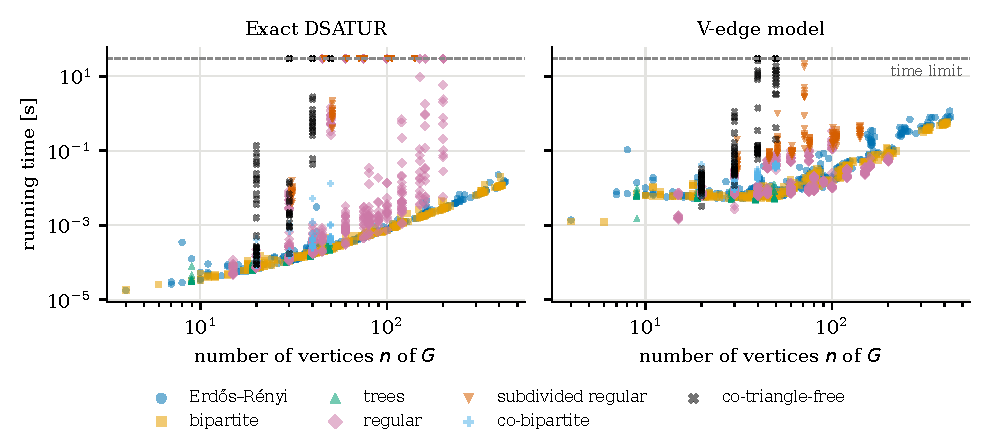
\includegraphics[width=0.74\textwidth]{figures/fig_time_vs_n}
\caption{Running time of exact coloring against the number of vertices.}
\label{fig:time}
\end{figure}

\subsection{Vertex coloring of $L(H)$ and edge coloring of $H$ (RQ2)}

All three models solved all $1125$ line graphs, so the comparison in
Table~\ref{tab:speedup} is complete. \Estar{} was faster than \Vedge{} on $91\%$
of the graphs (Wilcoxon test on logarithms of the times, $p<10^{-100}$), which
supports H1. The typical gain is moderate: the median of $S$ is $1.60$
(quartiles $1.17$ and $2.53$). If the reconstruction time is added, the root
approach is faster on $71\%$ of the graphs and the median of $S_{\mathrm{tot}}$
is $1.23$ (quartiles $0.98$ and $1.80$). For the whole set the three models
needed $145$\,s, $143$\,s and $69$\,s, and all reconstructions took $6.8$\,s.

\begin{table}[!tb]
\centering\small
\caption{Line graphs of set A: median times of the three models and of the root
reconstruction, and the speed-ups $S$ and $S_{\mathrm{tot}}$ (median), by family of
the root and by $R=|E(H)|/|V(H)|$.}
\label{tab:speedup}
\resizebox{\textwidth}{!}{\begin{tabular}{lrrrrrrrrrr}
\toprule
 & & \multicolumn{4}{c}{Median time [ms]} & \multicolumn{4}{c}{$S=T_V/T_E$} & \\
\cmidrule(lr){3-6}\cmidrule(lr){7-10}
Group & Graphs & $T_V$ & $T_C$ & $T_E$ & $T_{\mathrm{rec}}$ & Median & Geo.\ mean & Max & $S>1$ [\%] & $S_{\mathrm{tot}}$\\
\midrule
Erd\H{o}s--R\'enyi & 285 & 17.0 & 10.3 & 8.1 & 3.4 & 1.99 & 2.41 & 12.4 & 95 & 1.44\\
bipartite & 240 & 13.1 & 8.0 & 7.5 & 3.0 & 1.81 & 1.98 & 7.1 & 95 & 1.27\\
trees & 75 & 5.6 & 5.2 & 5.1 & 1.0 & 1.12 & 1.11 & 1.9 & 84 & 0.93\\
regular & 390 & 14.1 & 9.8 & 7.7 & 2.3 & 1.58 & 1.62 & 6.0 & 94 & 1.23\\
subdivided regular & 135 & 165 & 216 & 134 & 2.9 & 1.25 & 1.24 & 100.1 & 70 & 1.22\\
\midrule
$R\le 1.5$ & 299 & 6.3 & 5.7 & 5.3 & 1.0 & 1.16 & 1.17 & 7.8 & 88 & 0.96\\
$1.5<R\le 3$ & 451 & 15.1 & 9.6 & 8.4 & 2.2 & 1.59 & 1.50 & 100.1 & 90 & 1.22\\
$3<R\le 6$ & 285 & 52.3 & 25.1 & 17.9 & 5.2 & 2.61 & 2.28 & 7.0 & 93 & 1.82\\
$R>6$ & 90 & 428 & 165 & 69.0 & 28.9 & 6.60 & 6.77 & 12.4 & 100 & 4.51\\
\midrule
All line graphs & 1125 & 16.7 & 10.3 & 8.5 & 2.5 & 1.60 & 1.77 & 100.1 & 91 & 1.23\\
\bottomrule
\end{tabular}
}
\end{table}

The gain depends on the root graph (Figure~\ref{fig:speedup}). $S$ is
positively correlated with $R$ ($\rho=0.71$) and with $\Delta(H)$
($\rho=0.70$), as expected in H2. The relation holds also within the families
($\rho=0.89$ for bipartite and $0.88$ for Erd\H{o}s--R\'enyi roots) and between
the $75$ parameter combinations of set A ($\rho=0.82$ for the medians of $S$
and $R$). For $R\le 1.5$ the median of $S$ is $1.16$ and that of
$S_{\mathrm{tot}}$ is $0.96$; for $R>6$ they are $6.60$ and $4.51$, and \Estar{}
is faster on every instance. The sizes of the models explain this: the median
numbers of constraint sets $|\mathcal{Q}|$ are $240$ for \Vedge, $40$ for
\Vclique{} and $26$ for \Estar, and the difference grows quadratically with the
degrees of $H$. For sparse roots, such as trees, the models have similar size,
and the reconstruction does not pay off ($S_{\mathrm{tot}}=0.93$).

The \Vclique{} model shows where the gain comes from. Clique constraints
computed from $G$ alone remove most of the difference: the median of
$T_C/T_E$ is $1.17$, and \Estar{} is faster than \Vclique{} on $85\%$ of the
graphs. The remaining advantage of the root graph is that the Krausz partition
is a small family of cliques covering all edges, and that Vizing's theorem
saves the second solver call for class~II roots. In practice the
reconstruction is a fast way to obtain a compact clique formulation.

Subdivided regular graphs behave differently. Their times vary by two orders
of magnitude between instances of the same size, \Vclique{} is often the
slowest model, and $S$ ranges from $0.04$ to $100$. Ten of the twelve instances
with $S<0.5$ belong to this family, and within it $S$ is not correlated with
$R$. The decisive step is the infeasibility proof for $k=\Delta$, and its
length seems to depend more on the branching of the solver than on the
formulation.

\begin{figure}[!tb]
\centering
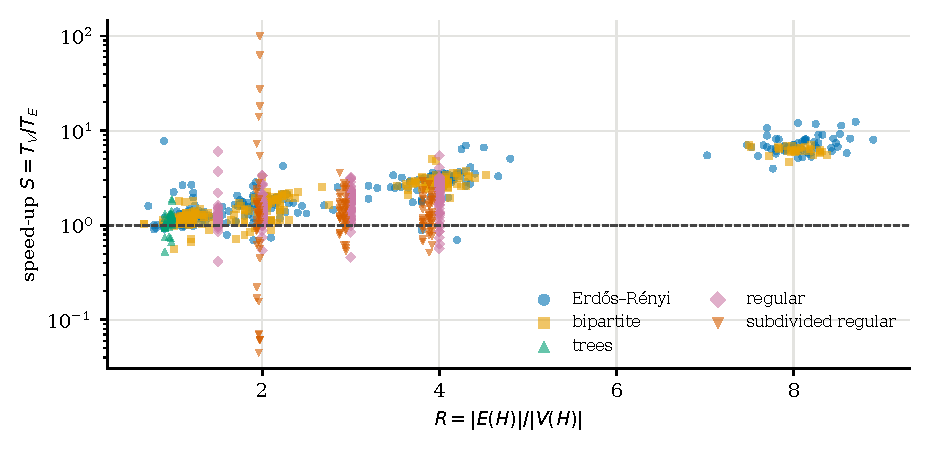
\includegraphics[width=0.64\textwidth]{figures/fig_speedup_vs_R}
\caption{Speed-up $S=T_V/T_E$ against $R=|E(H)|/|V(H)|$ for the line graphs of
set A (logarithmic vertical axis).}
\label{fig:speedup}
\end{figure}

\subsection{Class I and class II roots}

Set A contains $899$ line graphs of class~I roots and $226$ of class~II roots:
$90$ regular graphs of odd order (overfull), the $135$ subdivided regular graphs
of Observation~\ref{obs:subdiv}, and one cubic graph on ten vertices that is
neither. Table~\ref{tab:classes} shows that, within the tested families, the
class of the root has a large effect. In the regular and subdivided regular
families, where orders and degrees are comparable, the median of $T_V$ rises
from $9.9$\,ms for class~I to $94.8$\,ms for class~II, and the median of $T_E$
from $6.8$\,ms to $68.4$\,ms (Mann--Whitney test, $p<10^{-70}$ in both cases).
For DSATUR the effect is much stronger: it solved $99.1\%$ of the class~I
instances but only $27.0\%$ of the class~II ones.

The overfull instances were easier for the integer programming models than
the subdivided graphs, which are not overfull. For every pair $(n_0,d)$ with
$n_0\in\{15,25\}$, the median times of \Vedge{} and \Estar{} on the regular
graphs were $1.4$ to $2.8$ times smaller than on the corresponding subdivided
graphs. The hardest group, subdivided $4$-regular graphs with $n_0=35$, had
median times of $2.7$\,s for \Vedge{} and $0.52$\,s for \Estar, with maxima of
$22.3$\,s and $7.6$\,s.

\begin{table}[!tb]
\centering\small
\caption{Line graphs of set A by the class of the root graph.}
\label{tab:classes}
\resizebox{\textwidth}{!}{\begin{tabular}{llrrrrrrr}
\toprule
 & & & \multicolumn{2}{c}{Exact DSATUR} & \multicolumn{3}{c}{Median model time [ms]} & \\
\cmidrule(lr){4-5}\cmidrule(lr){6-8}
Class of $H$ & Family & Graphs & Solved [\%] & Median nodes & $T_V$ & $T_C$ & $T_E$ & Overfull [\%]\\
\midrule
I & Erd\H{o}s--R\'enyi & 285 & 100.0 & 0 & 17.0 & 10.3 & 8.1 & 0\\
I & bipartite & 240 & 100.0 & 0 & 13.1 & 8.0 & 7.5 & 0\\
I & trees & 75 & 100.0 & 0 & 5.6 & 5.2 & 5.1 & 0\\
I & regular & 299 & 97.3 & 106 & 9.9 & 8.1 & 6.8 & 0\\
I & all families & 899 & 99.1 & 0 & 10.3 & 8.0 & 6.8 & 0\\
\midrule
II & regular & 91 & 34.1 & 5006080 & 55.6 & 58.8 & 36.0 & 99\\
II & subdivided regular & 135 & 22.2 & 5055488 & 165 & 216 & 134 & 0\\
II & all families & 226 & 27.0 & 5054592 & 94.8 & 121 & 68.4 & 40\\
\bottomrule
\end{tabular}
}
\end{table}

\subsection{Structural parameters and difficulty (RQ3)}

Table~\ref{tab:corr} gives Spearman's correlations between structural
parameters and three measures of difficulty. The size of the DSATUR search tree
is only weakly related to the size of the graph ($\rho\approx 0.2$ for $n$ and
$m$), but it is strongly associated with the chromatic gap under the
implemented search strategy: $\rho=0.77$ on set A and $\rho=0.95$ on set B. This
is partly a consequence of the algorithm itself. If the heuristic finds an
$\omega$-coloring, the search stops at once; if $\chi>\omega$, the lower bound
$\omega$ can never close the gap. The association remains within single
families ($\rho=0.68$ for regular roots, $0.76$ for co-triangle-free graphs).
The running times of the integer programming models are related mainly to
size: for $T_V$ the strongest correlates are $m$ ($\rho=0.82$), the degeneracy
($0.76$) and $n$ ($0.75$), and the gap follows with $0.50$. For $T_E$ the gap
($0.61$) is as strongly associated as the degeneracy ($0.61$) and $n$
($0.63$), because the compact model removes much of the effect of size.
Density and $D_N$ show weak associations in all cases.

These parameters are themselves correlated (for example, the degeneracy grows
with $m$), so a single coefficient does not show which of them causes the
difficulty. H3 is therefore confirmed only in part. The gap is clearly more
closely related than $n$ to the work of branch and bound, the degeneracy is
about as good as $n$ and $m$ for the models, and $D_N$ is not informative in a
class where it is always high. The gap is also known only after the problem
has been solved. For line graphs it is determined by the class of the root,
and only sufficient conditions, such as overfullness, are cheap to test.

\begin{table}[!tb]
\centering\small
\caption{Spearman's $\rho$ between structural parameters and measures of
difficulty. $T_V$ on set B is restricted to solved instances; node counts of
runs stopped at the time limit are the counts at interruption. Values marked
with $^{\circ}$ are not significant at the level $0.001$.}
\label{tab:corr}
\begin{tabular}{lrrrrr}
\toprule
 & \multicolumn{3}{c}{Set A (line graphs)} & \multicolumn{2}{c}{Set B (non-line)}\\
\cmidrule(lr){2-4}\cmidrule(lr){5-6}
Parameter & $T_V$ & $T_E$ & DSATUR nodes & $T_V$ & DSATUR nodes\\
\midrule
$n$ & $+0.75$ & $+0.63$ & $+0.16$ & $+0.67$ & $+0.20$$^{\circ}$\\
$m$ & $+0.82$ & $+0.68$ & $+0.19$ & $+0.68$ & $+0.21$$^{\circ}$\\
density & $-0.13$ & $-0.10$$^{\circ}$ & $-0.01$$^{\circ}$ & $+0.35$ & $+0.10$$^{\circ}$\\
$\Delta(G)$ & $+0.66$ & $+0.49$ & $-0.11$ & $+0.63$ & $+0.13$$^{\circ}$\\
$\omega(G)$ & $+0.62$ & $+0.45$ & $-0.18$ & $+0.41$ & $-0.23$\\
$\chi-\omega$ & $+0.50$ & $+0.61$ & $+0.77$ & $+0.66$ & $+0.95$\\
degeneracy & $+0.76$ & $+0.61$ & $+0.20$ & $+0.70$ & $+0.25$\\
$D_N(G)$ & $+0.35$ & $+0.21$ & $-0.20$ & $+0.28$ & $-0.03$$^{\circ}$\\
\bottomrule
\end{tabular}

\end{table}

\section{Discussion}

The answer to RQ2 is positive, with reservations. With the reconstruction
included, the root approach was faster on $71\%$ of the line graphs and on all
graphs with dense roots, while for sparse roots it gave no gain. The conflict
structure of $L(H)$ is then described by $|V(H)|$ stars instead of
$\sum_v\binom{d_H(v)}{2}$ edges. The \Vclique{} model shows that most of this
gain is the known advantage of clique constraints over edge constraints. What
the root graph adds is a compact clique cover obtained in linear time and the
restriction of the search to one value of $k$. It does not make hard instances
easy: proving that a class~II graph has no $\Delta$-edge-coloring is the most
expensive step in every formulation.

For RQ1, the experiments suggest that the difference between easy and hard
instances depends less on whether a graph is a line graph than on whether
$\chi=\omega$. In line graphs Vizing's theorem keeps the gap at most one. In
complements of triangle-free graphs the gap can be large, and both general
methods failed on some of them at $50$ vertices, although a matching algorithm
colors them optimally. In both parts of the class, knowledge of the structure
helps, but the relevant structure is different.

\paragraph{Limitations.}
(i) Only one integer programming solver with default settings was used; a
constraint programming solver with \texttt{AllDifferent} propagation, such as
CP-SAT \cite{perron2023}, may rank the models differently. The software
contains such a back-end, but it was not used in the reported experiments.
(ii) DSATUR is written in pure Python and lacks the improvements of
\cite{sansegundo2012,furini2017}, so its times are pessimistic and the
comparison with HiGHS concerns these implementations only. (iii) Most
instances are solved within milliseconds, where timing noise is not
negligible. (iv) Set B consists of two dense families with $\alpha\le 2$; in
particular, it contains no quasi-line graphs that are not line graphs.
(v) Specialized exact solvers \cite{vanhoeve2022,heule2022,faber2024} are much
stronger than our baselines on general benchmarks and should be included in
further work.

\section{Conclusions}

We compared vertex coloring of line graphs with edge coloring of their
reconstructed roots, using DSATUR and three integer programming models on
three test sets of claw-free graphs. The main findings are:
\begin{enumerate}\setlength{\itemsep}{1pt}
\item The root model was faster than the edge model on $G$ for $91\%$ of
$1125$ line graphs (median speed-up $1.60$); with the reconstruction time
included, for $71\%$ (median $1.23$). The gain grows with $|E(H)|/|V(H)|$ and
reaches a median of $6.6$ for the densest roots (H1 and H2 supported).
\item Most of the advantage is already obtained with clique constraints
computed from $G$ (median times $16.7$, $10.3$ and $8.5$\,ms for \Vedge,
\Vclique{} and \Estar). The root graph adds a compact clique cover and the
two-valued bound of Vizing's theorem.
\item Within the tested families, line graphs of class~II roots were about ten
times slower for the integer programming models, and DSATUR solved only $27\%$
of them.
\item Among the tested claw-free graphs that are not line graphs, co-bipartite
graphs were easy, and the co-triangle-free family contained the hardest
instances of the study.
\item Under the implemented search strategy, the chromatic gap is the
parameter most strongly associated with the size of the DSATUR search tree,
while the times of the integer programming models follow the size and
degeneracy of the graph (H3 supported in part).
\end{enumerate}
Further work may include a constraint programming solver and current
SAT-based coloring solvers \cite{heule2022,faber2024}, cheap structural tests
(K\"onig's theorem, overfull subgraphs) in the root model, quasi-line graphs and
claw-free graphs with $\alpha\ge 3$, and a regression model that predicts the
running time from parameters known before solving.

\paragraph{Data availability.}
The source code, the instance generators with their seeds and the raw results
are available at \url{https://github.com/AnetaWrob/claw-free-graph-coloring}.

{\footnotesize
\setlength{\bibsep}{1pt}
\bibliographystyle{abbrvnat}
\bibliography{references}
}
\end{document}

